\documentclass[tikz, margin=30mm]{standalone}
\usepackage{tikz}
\usetikzlibrary{shapes.geometric, arrows, positioning, decorations.pathreplacing, calc, matrix, fit}
\usepackage[margin=0.5cm]{geometry}


\begin{document}

\begin{tikzpicture}[node distance=2cm and 2cm,
  % every node/.style={inner sep=0,outer sep=0}
  inner/.style={draw=black!80,fill=white!20,thick, inner sep=04pt},
  outer/.style={draw=black,fill=white!10,thick,inner sep=08pt},
  mymatrix/.style={matrix of nodes, nodes=typetag, row sep=1em},
  mycontainer/.style={draw=white, inner sep=1ex},
  typetag/.style={draw=white, inner sep=1ex, anchor=west},
  title/.style={draw=none, color=white, inner sep=0pt},
  ]

  \node[outer, remember picture,outer xsep=02pt] (input) {
    \begin{tikzpicture}
    \foreach \x in {1,...,4}
    {
      \node[yslant=0.5] (wsi\x) at (\x*.4,0) {
        \includegraphics[width=1.1cm, height=1.1cm]{./wsi\x.png}
      };
    }
  % Calculate the coordinates for the box
  \path (wsi1.south west) ++(0,-0.1) coordinate (bottom left);
  \path (wsi4.north east) ++(0,0.1) coordinate (top right);

  % Draw the box around the images
  \draw[black, thick] (bottom left) rectangle (top right);
  \node[below=0.0cm of bottom left, anchor=north west, align=center] (label) {Training Data};

    \foreach \x in {5,...,7}
    {
      \node[yslant=0.5] (wsi\x) at (3.5-\x*.4,-4) {
        \includegraphics[width=1.1cm, height=1.1cm]{./wsi\x.png}
      };
    }
  % Calculate the coordinates for the box
  \path (wsi5.south west) ++(-.8,-0.1) coordinate (bl2);
  \path (wsi7.north east) ++(.8,0.1) coordinate (tr2);

  % Draw the box around the images
  \draw[black, thick] (bl2) rectangle (tr2);
  \node[below=0.0cm of bl2, anchor=north west, align=center] (label2) {Test Data};


  \matrix[mymatrix, below=0.1cm of label2, draw] (mx1) {
    |[title]| \\
    % Labels \\
    Sensitive Variables \\
  };
  \node[below=0.0cm of mx1, text width=4.2cm, align=center] (label3) {Annotations};

\coordinate [below left=0.4cm and -1.90cm of label3] (Model) {};

\def\numLayers{5}
\def\offset{0.2}
\foreach \n in {1,...,\numLayers}
{
    \pgfmathsetmacro{\shiftX}{(\numLayers - \n) * \offset}
    \pgfmathsetmacro{\shiftY}{(\numLayers - \n) * \offset / 2}

    \draw[fill=blue!30, opacity=0.9] ([shift={(\shiftX, \shiftY)}]Model) rectangle ++(.4,-2);
}

      \node at ([shift={(2*\offset, -\numLayers*\offset - 1.5)}]Model) (ssl) {Model};

  \end{tikzpicture}
};

\coordinate [right=4 of input] (Overfit) {};
  \node[outer, remember picture] (Overfit) at (Overfit) {
    \begin{tikzpicture}

  \node[inner, remember picture] (finetune) {
    \begin{tikzpicture}
  \node[] (monai) {
    
\includegraphics[width=1.5cm, height=1.5cm]{./MONAI-logo-color.png}
  };

      \node[below=0.0cm of monai]  (pytorch) {
    
\includegraphics[width=1.5cm, height=1.5cm]{./Pytorch_logo.png}
  };
\end{tikzpicture} };
  \node[inner, remember picture, below=0.1cm of finetune] (labelFine) { Sensitive Variable TL };

  \node[below=0.0cm of labelFine, text width=4.2cm, align=center] (UMAP) {
    \begin{tikzpicture}
      \node[] (umap) {
        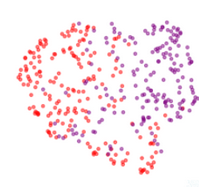
\includegraphics[width=1.5cm, height=1.5cm]{./simpleUmap.png}
      };
      \node[inner, remember picture, below=0.1cm of umap] (labelUmap) { UMAP };
    \end{tikzpicture}
    };

\node[inner, remember picture, below=0.4cm of UMAP] (fairness) { 
    \begin{tikzpicture}
  \node[] (fairness) { 
    \begin{tikzpicture}[line width=1mm, scale=.3]
        % Draw the base
        \draw (-3,0) -- (3,0);
        % Draw the vertical post
        \draw (0,0) -- (0,4);
        % Draw the horizontal beam
        \draw (-2,4) -- (2,4);
        % Draw the fulcrum
        \filldraw[black] (0,4) circle (4pt);
        % Draw the left scale
        \draw (-2,4) -- (-2.5,2);
        \draw (-2,4) -- (-1.5,2);
        \draw (-2.5,2) -- (-1.5,2);
        \draw (-1.5,2) arc[start angle=0,end angle=-180,radius=0.5];
        % Draw the right scale
        \draw (2,4) -- (1.5,2);
        \draw (2,4) -- (2.5,2);
        \draw (2.5,2) -- (1.5,2);
        \draw (2.5,2) arc[start angle=0,end angle=-180,radius=0.5];
      \end{tikzpicture}
    };
      \node[inner, remember picture, below=0.1cm of fairness] (labelFairness) { Fairness Measuring };
  \end{tikzpicture}
};
  \end{tikzpicture}
      };

\node[outer, remember picture, right=1.8 of Overfit] (output) {
    \begin{tikzpicture}

      \node[inner, remember picture, below=0.1cm of label3] (analysis) { Analysis Results };

      \node[inner, remember picture, below=0.1cm of analysis] (analysis) { Plots };
    \end{tikzpicture}
  };

\node [above=.0cm of input] (inputText) {Input};
\node [above=.0cm of Overfit] (overfitText) {Overfit detection plugin};
\node [above=.0cm of output] (outputText) {Output};

\draw[->] (input) -- (Overfit);
\draw[->] (Overfit) -- (output);
 
 
\end{tikzpicture}

\end{document}

